\documentclass{article}
\usepackage[a4paper, total={6in, 10in}]{geometry}
\setlength{\parskip}{0.01cm plus4mm minus3mm}

\usepackage{multicol}
\usepackage{enumitem}

\usepackage{listings}
\usepackage{xparse}

\usepackage[superscript,biblabel]{cite}
\usepackage{graphicx}
\usepackage{hyperref}
\usepackage{caption}

\usepackage{blindtext}
\usepackage{dirtree}

\usepackage{xcolor}
\colorlet{cBlue}{blue!80}
\colorlet{cPurple}{blue!40!red}
\colorlet{cRed}{red!60}

\NewDocumentCommand{\codeword}{v}{
    \texttt{\textcolor{cBlue}{#1}}
}

\NewDocumentCommand{\cmd}{v}{
    \textit{\textcolor{cPurple}{#1}}
}

% Styles stolen from https://www.overleaf.com/learn/latex/Code_listing
\definecolor{codegreen}{rgb}{0,0.6,0}
\definecolor{codegray}{rgb}{0.5,0.5,0.5}
\definecolor{codepurple}{rgb}{0.58,0,0.82}
\definecolor{backcolour}{rgb}{0.95,0.95,0.92}

\lstdefinestyle{mystyle}{
    backgroundcolor=\color{backcolour},   
    commentstyle=\color{codegreen},
    keywordstyle=\color{magenta},
    numberstyle=\tiny\color{codegray},
    stringstyle=\color{codepurple},
    basicstyle=\ttfamily\footnotesize,
    breakatwhitespace=false,         
    breaklines=true,                 
    captionpos=b,                    
    keepspaces=true,                 
    numbers=left,                    
    numbersep=5pt,                  
    showspaces=false,                
    showstringspaces=false,
    showtabs=false,                  
    tabsize=2
}

\lstset{style=mystyle}

\title{World of Deez}
\author{Pawel Makles \\ \small (K21002534)}
\date{\small Created: 19th November 2021 \\ Last Modified: 3rd December 2021}

\begin{document}
\maketitle

    \begin{multicols}{2}
        \section{User Level Description}
        This game is largely open world but has a main storyline which the player can choose to follow to complete the game, as well as other side-quests which can be done alongside or after the story.

        In this game, you are one of millions of citizens in an isolated city home to a Beastman \cite{beastman} society, the city being loosely based off Animacity \cite{animacity} from the series Brand New Animal \cite{bna}. The plot revolves around Sylvasta who is deeply intertwined with the city and owns the city's medical centre.

        There have been reports that their research has been highly unethical and leaks have been coming out from former employees which have been riling up protests throughout the city. Your goal is to figure out what's really happening and to put a stop to it.

        I ended up not adding any information about the main character as to add to the open world, `your adventure', feeling. The story is also loosely based off Utopia \cite{utopia}, in which a group of people find out the truth behind a manuscript and find themselves in the middle of a conspiracy \cite{pyrocynical}.
        
        \section{Implementation}
        The project is split up into several packages, most of which work independently of each other, in general, the \codeword{Game} uses the \codeword{commands} package (providing actions the player can perform) along with the \codeword{world} (providing the things that the player can interact with in the game) package to run the game. They are laid out as follows:
        
            \subsection{Commands}
            This package provides the classes required to parse and run commands, it includes the \codeword{CommandManager} which registers objects of type \codeword{Command}. More about parsing commands is in the challenge task section.

            This package also includes a subpackage called \codeword{core} containing all of the `core' commands required to run any game world, this includes things such as picking items up, quiting the game, and so forth.
            
            \subsection{Entities}
            This package provides the basic tools required to create simple and complex entities within the world, more about entity detail is discussed later.

            It also contains a subpackage \codeword{actions} which contains common interfaces which entities can implement to allow the ways that they can be interacted with to be quite modular.
            
            \subsection{Content / Campaign}
            The \codeword{content.campaign} package contains a lot of custom content derived from the base game used to construct the story and the story world.
            
            \subsection{World}
            This package has the basic building blocks for creating worlds including the \codeword{World} and \codeword{Room} classes which can be easily extended for more functionality. The only limitations are that traveling between rooms must be done in a direction specified in the \codeword{Direction} enum and that the \codeword{Location} of any entity must be either a room, inventory or neither.
            
            \subsection{Util}
            This package contains a bunch of small utility classes, including:

                \begin{itemize}[leftmargin=*]
                    \item \textbf{BlueJ.java} \cite{bluej}: Contains improved methods on detecting whether the application is currently running in BlueJ. (taken from my previous coursework assignment)
                    \item \textbf{Localisation.java}: A pretty straightforward implementation of a localisation engine. Simply maps (period-separated) keys to their respective (nested) keys in a language file.
                    \item \textbf{Search.java}: Methods for searching through various data structures in the game.
                    \item \textbf{Tree.java}: A very simple implementation of a tree with basic traversal methods.
                \end{itemize}

            \subsection{Dialogue \& IO \& UI \& Events}
            These are all discussed later on in the challenge task section.

        \section{Base Tasks}

            This section describes how I implemented the basic task requirements.

            \begin{itemize}[leftmargin=*]
                \item \textit{``The game has several locations the player can walk through.''}
                
                    I began by first designing the world map (see \autoref{fig:map}), using Excalidraw \cite{excalidraw}, then implemented each location as a \codeword{Room}.

                    To build the world, I made a \codeword{World} class to house all the locations which exist in the game world and then extended this using the \codeword{CampaignWorld} class which builds the story world, creates rooms and registers events.

                    I ended up adding $10$ locations into my game:
                    \begin{itemize}[leftmargin=*]
                        \item \textbf{City Centre}: Centre of the city connecting major areas with the coast.
                        \item \textbf{Apartments}: This is the player's residence.
                        \item \textbf{Street}: This is the main city street connecting important buildings.
                        \item \textbf{Shop}: The local city shop where the player frequents to get necessary items.
                        \item \textbf{Back Alley}: This is where the player can start the main story mission.
                        \item \textbf{Coastline}: There are two coasts, one on the city side and one on the mainland.
                        \item \textbf{Forest}: The forest grants access to the Worm Hole and to other side-quests.
                        \item \textbf{Worm Hole}: For challenge task 3.
                    \end{itemize}

                    The layout is heavily inspired by Animacity, although since there's no available map of the actual city, I made my own interpretation based off various pieces of art, (see \autoref{fig:runaway-raccoon}). I used an existing real life location to determine the size of the river \cite{river-map}.

                \item \textit{``There are items in some rooms that may or may not be picked up by players.''}
                
                    To achieve this, I considered all entities to be items which may or may not be picked up by other entities, each entity has its own \codeword{Inventory} which is in effect a list of other entities which it is holding.
                
                \item \textit{``Each item has a weight and the player can only carry items up to a certain weight.''}
                
                    To do this, I added a new private field \codeword{weight} of type double to the \codeword{Entity} class, which is used to store the entity's weight. It is a double as I wanted access to fractional weights (say $0.01$kg) and I wanted to have access to \codeword{Stream::mapToDouble} for summations.

                    For the second part, I made it so each \codeword{Inventory} has a maximum weight it can store, which by default is set to $0$ as each entity has an inventory but may not necessarily have the ability to store anything.

                    When putting anything in an inventory, we check that the following is satisfied:
                    $$
                        \textsf{currentWeight} + \textsf{itemWeight} \le \textsf{maxWeight}
                    $$

                    To determine the weight of common items, I referred to a document I found online published by the City of York Council \cite{common-weights}.
                
                \item \textit{``Player can win.''}
                
                    The player may win by completing the main story mission (detailed in the walkthrough) which sets a flag that the game has been completed, the player may choose to keep playing in the open world or run \cmd{win} to end the game.

                \item \textit{``There is a command} \cmd{back} {which takes you back to the last room.''}
                
                    I added two new private fields to the player entity, which were \codeword{previousRooms} and \codeword{retreatingDirection}, these are used to store the path back through the room and the direction which we need to go to get back there respectively. The direction is stored in order to run a check whether the player can actually go back in the direction they intend to, to verify this, the `retreating direction' is used to call the method \codeword{canLeave} on the current room the player is in.

                \item \textit{``Add at least four new commands.''}
                
                    I added several additional commands which are listed below:

                    \begin{itemize}[leftmargin=*]
                        \item \cmd{bag}: Allows the player to look at their or another entity's inventory.
                        \item \cmd{drop}: Drop any specified item from the player's inventory into current room.
                        \item \cmd{give}: Give a specified item to another entity, we ensure that the entity implements \codeword{IGiveable} and give the item to the entity using \codeword{IGiveable::give}.
                        \item \cmd{pet}: Pet a specified entity, has to implement \codeword{IPettable}, we use \codeword{IPettable::pet}.
                        \item \cmd{take}: Take any specified item from another entity's inventory.
                        \item \cmd{talk}: Initiate a conversation with an entity, must implement \codeword{ITalkwith}, we call \codeword{ITalkwith::talk} to start the conversation.
                        \item \cmd{use}: `Use' an entity, we call \codeword{IUseable::use} to use the entity. (implemented by entity)
                        \item \cmd{where am i}: Tells the game to print out room information again, this is done by emitting \codeword{EventEntityEnteredRoom} again.
                    \end{itemize}

                    See \autoref{fig:help-command} for an example of the help menu.
            \end{itemize}

        \setlength{\parskip}{0.1cm plus4mm minus3mm}
        \section{Challenge Tasks}

            This section describes how I implemented the challenge tasks and what I did in addition.

            \subsection{Required Tasks}
            \begin{itemize}[leftmargin=*]
                \item \textit{``Add characters to your game.''}
                
                    I ended up adding $8$ characters to my game, $3$ of which can move on their own.

                    \begin{itemize}[leftmargin=*]
                        \item \textbf{Static NPCs}: There are several static NPCs which the player can interact with, talk with or complete missions for.
                        Including the receptionist, city NPC, the old man, the security guard, the shopkeeper and Marie who is part of the main story.
                        \item \textbf{Dynamic NPCs}: There are $2$ NPCs which appear or disappear depending on the state of the game, this includes the protestors and security guard.
                        \item \textbf{Moving NPCs}: There is a single NPC, the cat, which randomly follows a fixed path to move around the map. This is done by listening to \codeword{EventTick} from world events and then randomly deciding to move.
                    \end{itemize}

                    Note on character creation: I decided to stick to mostly generic characters in the game, mainly since the people you encounter have not as much impact on the story, with the exception of Marie \cite{marie}, who I took straight from BNA \cite{bna}, see \autoref{fig:festival-marie}, she is a sly and cunning character which I think perfectly fits the role I need.

                \item \textit{``Extend the parser.''}
                
                    I entirely replaced how the parser worked, I began by implementing a basic model of \codeword{Command}, it took a few iterations but I settled on providing Regex \codeword{Pattern}s.

                    This approach has several benefits:

                    \begin{itemize}[leftmargin=*]
                        \item Powerful Regex at low performance cost due to the low number of commands.
                        \item Ability to have named capture groups which are then interpreted as arguments.
                    \end{itemize}

                    For each known \codeword{Command}, I would create a \codeword{Matcher} for each \codeword{Pattern}, execute it against the arbitrary command from the user and then pass it into a wrapper class \codeword{Arguments} which lets me safely pull out named groups, directions or any other argument type I need.
                
                \item \textit{``Add a magic transporter room.''}
                
                    To do this, I added a \codeword{RoomWormHole} which I made implement \codeword{EventEntityEnteredRoom} to listen for when any entities entered the room, as soon as one is detected, a short animation is played and a room is selected at random to teleport the user to. Allowing the user to go to \textbf{any room} may interfere with my story so I chose to only spawn the user at any outside areas of the map.
                \end{itemize}

                \subsection{World Event System}
                \textit{``Add a system for managing world events.''}

                    I began by creating a basic \codeword{Event} class which can be extended to hold any arbitrary data, it also provides basic functionality to prevent event propagation (see \autoref{fig:event}).

                    I created an \codeword{EventSystem} class which would manage incoming and outgoing events, I decided that it should have the ability to handle any event and allow anything to create listeners for any object that extends Event.

                    To map these, I had a \codeword{HashMap} which mapped unique \codeword{Class<? extends Event>} to linked (as to keep order of registration) hash sets of \codeword{IEventListener<? extends Event>}. The interface simply provides a single method, \codeword{onEvent(Event e)}, which is called when the event is triggered.

                    Since Java has type erasure, it means my generic type annotations are gone once the program is compiled, so I can't do things such as object is `instanceof' class. As such, I decided to ignore cast warnings and entirely rely on compiler type checking to verify that the objects provided are correct, I achieved this by adding a generic type argument to the add listener method and making the compiler check that the target class and event listener match, see \autoref{fig:generic-method}.

                \subsection{Dialogue}
                \textit{``Give NPCs interactive dynamic dialogue.''} \\

                    To implement dialogue, I made a simple data structure implemented as follows:

                    \dirtree{%
                        .1 Dialogue.
                        .2 DialogueNode.
                        .3 DialogueOption.
                        .3 DialogueOption.
                        .2 DialogueNode.
                        .3 DialogueOption.
                    }

                    The \codeword{Dialogue} houses several nodes each of which have options which lead to other nodes. With this system, I can add dynamic conversations, such as with the shopkeeper, by extending the \codeword{DialogueNode} class and providing my own dynamically generated description and options.

                    For simpler tasks, such as changing game state through conversation, I can create a new \codeword{DialogueOption} with an \codeword{IDialogueHandler} which provides a method that the dialogue system calls to determine whether anything else needs to happen and what the next node is.

            \setlength{\parskip}{0.01cm plus4mm minus3mm}

                \subsection{Terminal Emulator}
                \textit{``Implement a terminal emulator.''} \\

                I began by creating a new \codeword{IOSystem} interface which provides common I/O methods, such as \codeword{print}, \codeword{println} and \codeword{readLine}. I then made all game output come through this interface and created two new classes that implemented it, \codeword{StandardIO} as a fallback to stdout and the \codeword{TerminalEmulator} which creates a new window. \\

                To render the window I have a class extending \codeword{JFrame} which shows my \codeword{JTerminalView}. To render the text I override into \codeword{paintComponent} and draw my own content using the provided \codeword{Graphics} context \cite{code-ref-7}. (example: \autoref{fig:terminal}) \\

                The font used is VT323 Regular \cite{font}.

                    \subsubsection{Ansi Escape Codes}

                        One of the main reasons I built this was for greater flexibility, so naturally I added support for Ansi escape codes. I matched the escape codes in the \codeword{TextBuffer} and adjusted the buffer accordingly. (\autoref{fig:ansi-match} for the implementation)

                    \subsubsection{Emoji Support}

                        I also added a way to load and display small images like emojis (see \autoref{fig:emoji}), although I had some difficulties with Unicode being mangled when working with BlueJ \cite{bluej-issue}.

                    \subsubsection{EventDraw and the Map}

                        Since I already had a way to load images, I also provided a way for anything to draw to the terminal. I added an \codeword{EventDraw} (\autoref{fig:event-draw}) which is emitted whenever the terminal view paints and used it to draw a map (see \autoref{fig:map-ingame}).

        \section{Code Quality}
        % For each of the following code quality considerations, give and explain an example in your
        % project where you considered it: coupling, cohesion, responsibility-driven design, maintain-
        % ability.

            \subsection{Coupling}
                % The term coupling describes the interconnectedness of classes. We strive for 
                % loose coupling in a system—that is, a system where each class is largely independent and 
                % communicates with other classes via a small, well-defined interface.
                An example of loose coupling in my project is the \codeword{EventSystem}, it is completely independent from the rest of the project and can be used with anything (see \autoref{fig:event-system}), as such I am using it with both the \codeword{World} and \codeword{TerminalEmulator} for different purposes to provide different sets of events. Another example of loose coupling is the \codeword{Dialogue<T>} system, it accepts any kind of key through the generic \codeword{T} so it can be used with practically anything and if needed, the type can be constricted (example: \autoref{fig:dialogue}). The only dependency it has is the \codeword{IOSystem} interface.

            \subsection{Cohesion}
                % The term cohesion describes how well a unit of code maps to a logical task 
                % or entity. In a highly cohesive system, each unit of code (method, class, or module) is 
                % responsible for a well-defined task or entity. Good class design exhibits a high degree of cohesion.
                One example of high cohesion is the \codeword{IOSystem} interface (see \autoref{fig:io-system}) and the classes which implement it. It is used throughtout the project to refer to an arbitrary input or output, as such, the first implementation I made was StandardIO (see \autoref{fig:standard-io}) which passes these methods through to \codeword{System.out/in}. One benefit is that I can easily slot in additional processing layers, such as \codeword{LocalisedIO} (see \autoref{fig:localised-io}) which can take in data, process it and pass it through to an arbitrary \codeword{IOSystem}.

            \subsection{Responsibility-driven design}
                % Responsibility-driven design is the process of designing
                % classes by assigning well-defined responsibilities to each class. This process can be used to 
                % determine which class should implement which part of an application function
                I considered responsibility-driven design when first building the structure of my project, for example, the \codeword{World} class is responsible entirely for keeping track of rooms and entities and nothing else, to add functionality to it you must extend it as I have done with the \codeword{CampaignWorld}. As another example, each \codeword{Entity} just stores any information directly relating to the entity such as a name and its location, to implement additional actions such as `using the entity', we must extend \codeword{Entity} and then implement \codeword{IUseable}.

            \subsection{Maintainability}
                % Writing for maintainability is maybe the most fundamental topic. It is about trying to write 
                % code in such a way that errors are avoided in the first place and, if they still slip in, that 
                % they can be found as easily as possible.
                One example of where I considered maintainability is the \codeword{Inventory} system, the logic is entirely self-contained and quite simple to understand. Fields such as \codeword{items}, \codeword{maxWeight} are both private and inaccessible outside of the inventory class, as such I can guarantee that the inventory always stays consistent and hence easily maintainable, these values may only be modified by methods with distinct tasks and appropriate validity checks (examples: \autoref{fig:inventory}).

        \section{Walkthrough}
            \textbf{\color{cRed}This guide will skip over some parts of the plot}, it serves as a way to just get to the end, I would recommend playing through first and then falling back on this if you are stuck. \\

            You wake up in your home, \cmd{go down}, then \cmd{east} then \cmd{north}. Here, you must \cmd{talk to Marie}, go through the prompts ($1 \rightarrow 1 \rightarrow 2 \rightarrow 1$) to progress the story. \\

            Now, \cmd{go south}, \cmd{north west}, \cmd{north} and \cmd{talk with shopkeeper}, buy the communicator device and leave. Now \cmd{go south}, \cmd{east}, \cmd{north} and \cmd{talk to Marie} again. Continue by going \cmd{south}, \cmd{north west}, \cmd{west}. Sit down by \cmd{use couch} then \cmd{use comms} and go through the prompts, afterwards \cmd{go down}. Here, you must pick up documents $2$, $4$ and $5$ by using \cmd{take doc2}, ... \\

            Now, \cmd{go up}, \cmd{east}, \cmd{south}, \cmd{up} to get back to your home and \cmd{use the laptop}. Go through the prompts ($1 \rightarrow 4 \rightarrow 2$). At this point, you can use the command \cmd{win}. If you want to do the side-quest, you'll have to figure it out yourself :-)

            \subsection{Access to teleporter room}
            To get to the teleporter room, you must go to the shopkeeper and buy the `speed boat key', from there you can go to the south of the city and use the boat to get to the mainland. Going south to the forest then east to get to the teleporter room.

        \section{Known Issues}
        
            \begin{itemize}[leftmargin=*]
                \item Anything starting with `b' will show inventory.
                \item NPC dialogue not changing between chapters.
                \item Can't include Unicode in Java source.
            \end{itemize}

    \end{multicols}

    \newpage

    \begin{thebibliography}{9}
        \bibitem{beastman}
        Brand New Animal Wiki. Beastman \\
        \url{https://brand-new-animal.fandom.com/wiki/Beastman}
        \bibitem{animacity}
        Brand New Animal Wiki. Animacity \\
        \url{https://brand-new-animal.fandom.com/wiki/Anima_City}
        \bibitem{marie}
        Brand New Animal Wiki. Marie Itami \\
        \url{https://brand-new-animal.fandom.com/wiki/Marie_Itami}
        \bibitem{bna}
        IMDb. BNA (TV Mini Series 2020) \\
        \url{https://www.imdb.com/title/tt12013558/}
        \bibitem{utopia}
        IMDb. Utopia (TV Series 2013-2014) \\
        \url{https://www.imdb.com/title/tt2384811/}
        \bibitem{excalidraw}
        Excalidraw. \\
        \url{https://excalidraw.com/}
        \bibitem{bluej}
        GitHub. maven-bluej / BlueJ.java \\
        \url{https://github.com/KCLOSS/maven-bluej/blob/master/BlueJ.java}
        \bibitem{river-map}
        Google Maps. Jezioro Świerklaniec, Poland \\
        \url{https://www.google.com/maps/@50.4293559,18.9742453,16.12z}
        \bibitem{common-weights}
        PDF. Set of average weights for furniture, appliances and other items \url{https://democracy.york.gov.uk/documents/s2116/Annex\%20C\%20REcycling\%20Report\%20frnweights2005.pdf}
        \bibitem{pyrocynical}
        YouTube. The best (and worst) show you haven't seen \\ \url{https://youtu.be/PFx2QM0Z8Qo}
        \bibitem{bluej-issue}
        GitHub. BlueJ Bug Reproductions (wip) \\ \url{https://github.com/insertish/bluej-bug-demo}
        \bibitem{font}
        Fontsource. VT323 \\ \url{https://fontsource.org/fonts/vt323}

        \textbf{\\ References in code.}

        \bibitem{code-ref-1}
        \codeword{Ansi.java} StackOverflow. How to print color in console using System.out.println? \\
        \url{https://stackoverflow.com/a/5762502}
        \bibitem{code-ref-2}
        \codeword{LocalisedIO.java} StackOverflow. What is the equivalent of Regex-replace-with-function-evaluation in Java 7? \url{https://stackoverflow.com/a/27359491}
        \bibitem{code-ref-3}
        \codeword{JTerminalFrame.java} How to detect a key press in Java \\
        \url{https://stackoverflow.com/a/21970006}
        \bibitem{code-ref-4}
        \codeword{JTerminalView.java} How to "do something" on Swing component resizing? \\
        \url{https://stackoverflow.com/a/8917978}
        \bibitem{code-ref-5}
        \codeword{JTerminalView.java} Java Documentation. Font Concepts \\
        \url{https://docs.oracle.com/javase/tutorial/2d/text/fontconcepts.html}
        \bibitem{code-ref-6}
        \codeword{JTerminalView.java} Java Documentation. Java Thread Primitive Deprecation \url{https://docs.oracle.com/javase/1.5.0/docs/guide/misc/threadPrimitiveDeprecation.html}
        \bibitem{code-ref-7}
        \codeword{JTerminalView.java} StackOverflow. Drawing Canvas on JFrame \\
        \url{https://stackoverflow.com/a/17922749}
        \bibitem{code-ref-8}
        \codeword{TerminalEmulator.java} StackOverflow. Passing values between 2 threads without intrrrupting each other \url{https://stackoverflow.com/a/23413506}

        \textbf{\\ Libraries used:}
        \bibitem{library-1}
        \cmd{com.moandjiezana.toml} \url{https://github.com/mwanji/toml4j}
        \bibitem{library-2}
        \cmd{commons-io} \url{https://commons.apache.org/proper/commons-io}
        \bibitem{library-3}
        \cmd{kuusisto.tinysound} (fork by DrogoniEntity) \url{https://github.com/DrogoniEntity/TinySound}
        \bibitem{library-4}
        \cmd{com.projectdarkstar.ext.jorbis} \\
        \url{https://search.maven.org/artifact/com.projectdarkstar.ext.jorbis/jorbis}
        \bibitem{library-5}
        \cmd{com.googlecode.soundlibs.tritonus-share} \\
        \url{https://search.maven.org/artifact/com.googlecode.soundlibs/tritonus-share/0.3.7.4/bundle}
        \bibitem{library-6}
        \cmd{com.googlecode.soundlibs.vorbisspi} \\
        \url{https://search.maven.org/artifact/com.googlecode.soundlibs/vorbisspi/1.0.3.3/bundle}

        \textbf{\\ Sounds used:}
        \bibitem{sound-money-bag}
        Freesound. "Money Bag" by PhilSavlem (licensed under CC0) \\
        \url{https://freesound.org/people/PhilSavlem/sounds/338260/}
        \bibitem{sound-waves-1}
        Freesound. "bay of fundy 01.flac" by tim.kahn (licensed CC BY 3.0) \\
        \url{https://freesound.org/people/tim.kahn/sounds/127569/}
        \bibitem{sound-waves-2}
        Freesound. "bay of fundy 02.flac" by tim.kahn (licensed CC BY 3.0) \\
        \url{https://freesound.org/people/tim.kahn/sounds/127568/}
    \end{thebibliography}
    
    \newpage

    % Appendix
    \captionsetup{justification=centering,margin=3cm}
    \begin{figure}
        \centering
        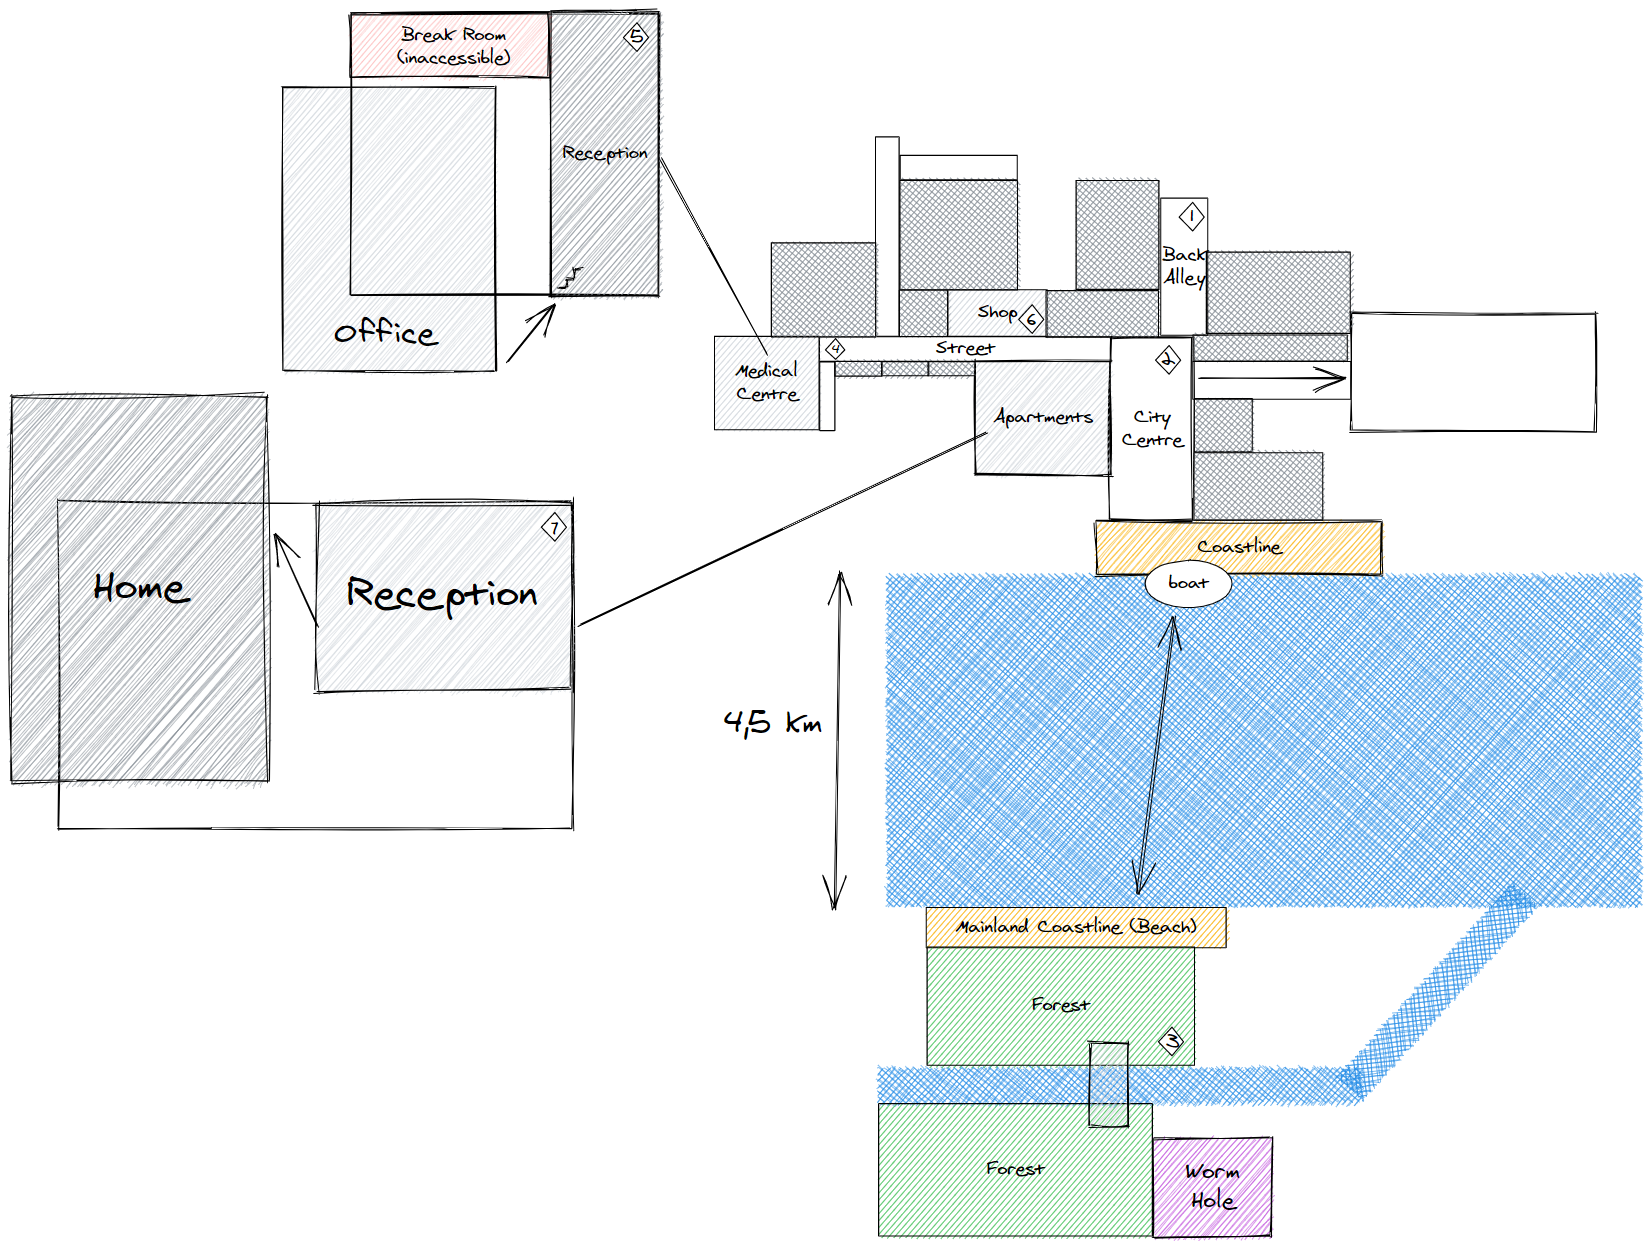
\includegraphics[width=\textwidth]{../src/main/resources/map/base.png}
        \caption{World Map} \label{fig:map}
    \end{figure}
    \begin{figure}
        \centering
        
\includegraphics[width=\textwidth]{images/runaway-raccoon-302.jpg}
        \caption{Shot of Animacity as seen in Episode 1 at 3:02 of Brand New Animal \cite{bna}} \label{fig:runaway-raccoon}
    \end{figure}
    \begin{figure}
        \centering
        
\includegraphics[width=\textwidth]{images/festival-marie.jpg}
        \caption{Michiru Kagemori and Marie Itami pictured left to right in Episode 1 at 12:51 of Brand New Animal \cite{bna}} \label{fig:festival-marie}
    \end{figure}
    \begin{figure}
        \centering
        
\includegraphics[width=\textwidth]{images/emoji.jpg}
        \caption{Sample emoji output} \label{fig:emoji}
    \end{figure}
    \begin{figure}
        \centering
        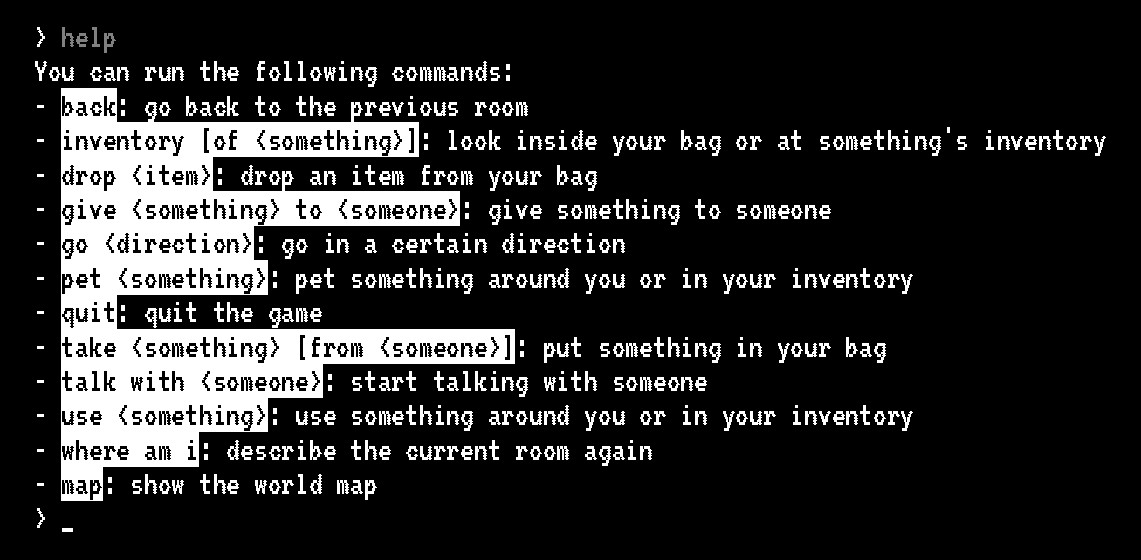
\includegraphics[width=\textwidth]{images/help-command.jpg}
        \caption{Output from the help command} \label{fig:help-command}
    \end{figure}
    \begin{figure}
        \centering
        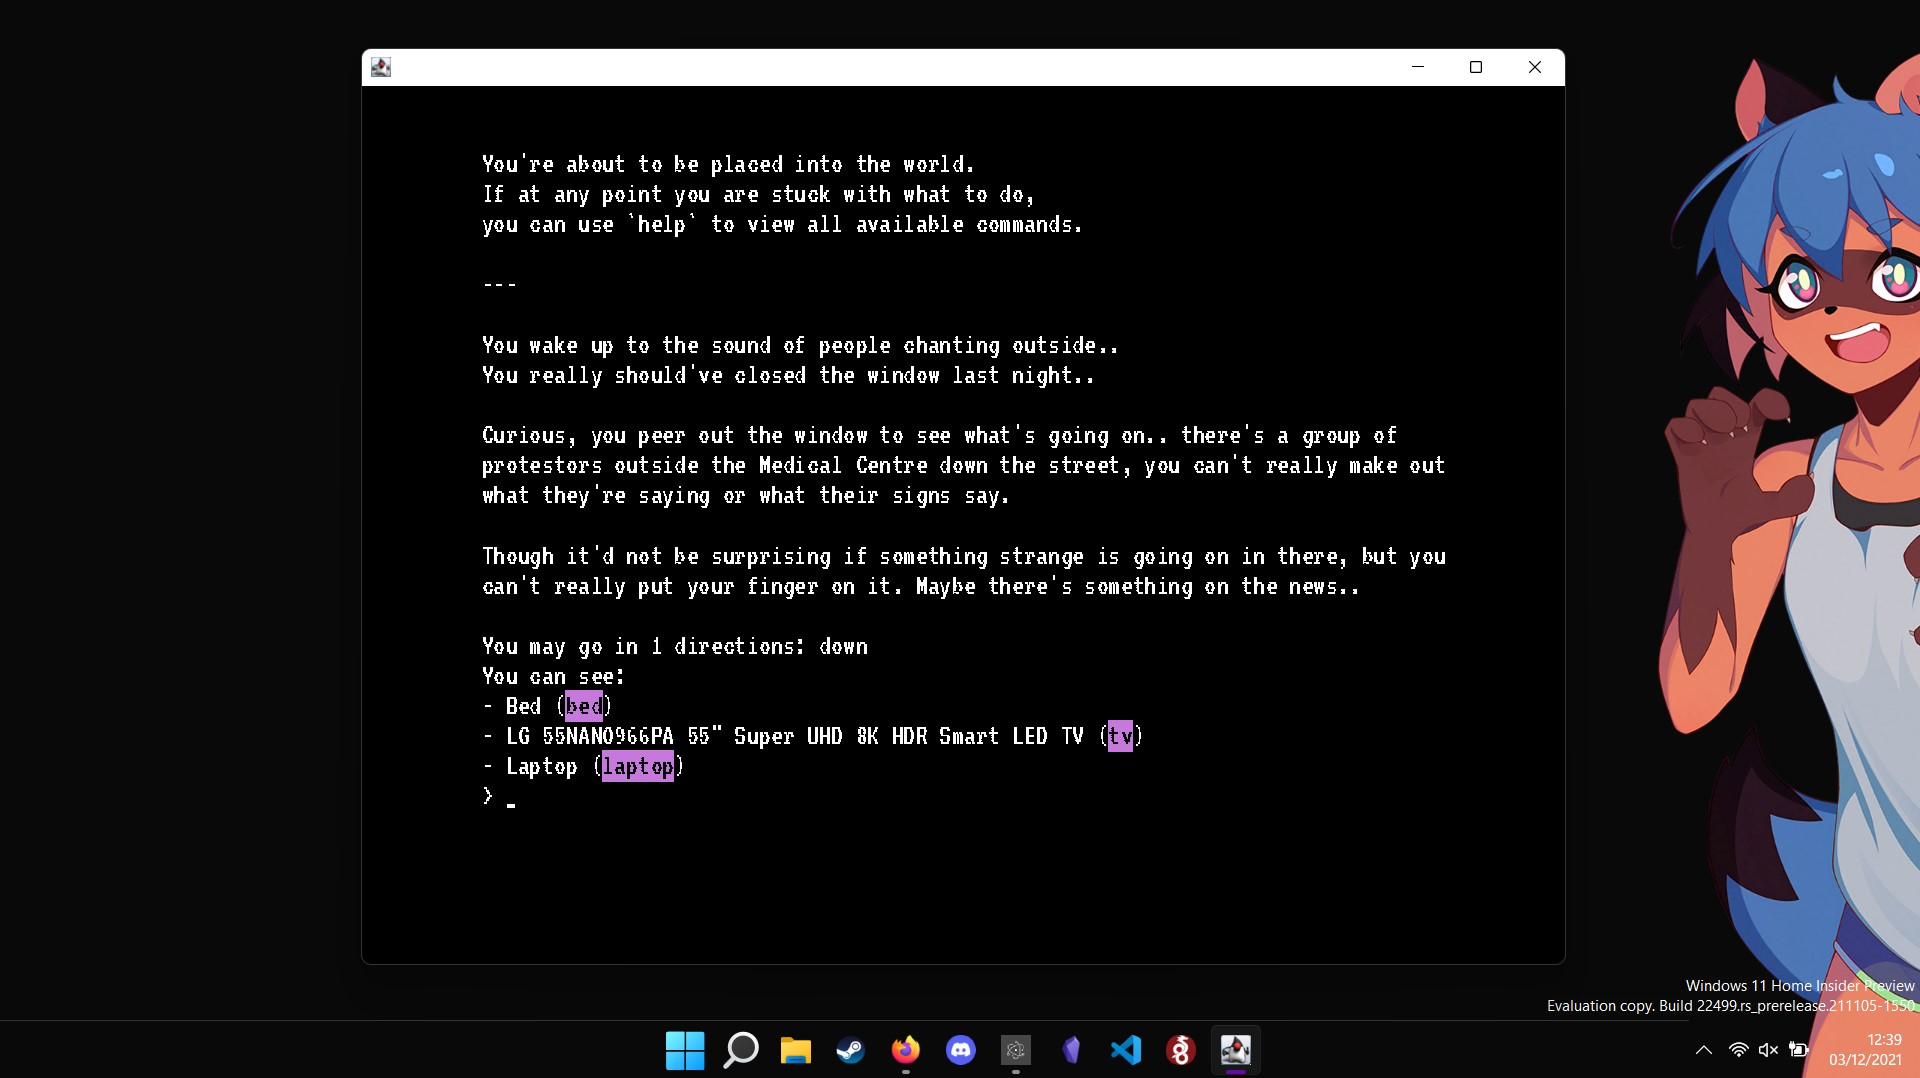
\includegraphics[width=\textwidth]{images/terminal.jpg}
        \caption{The terminal emulator} \label{fig:terminal}
    \end{figure}
    \begin{figure}
        \centering
        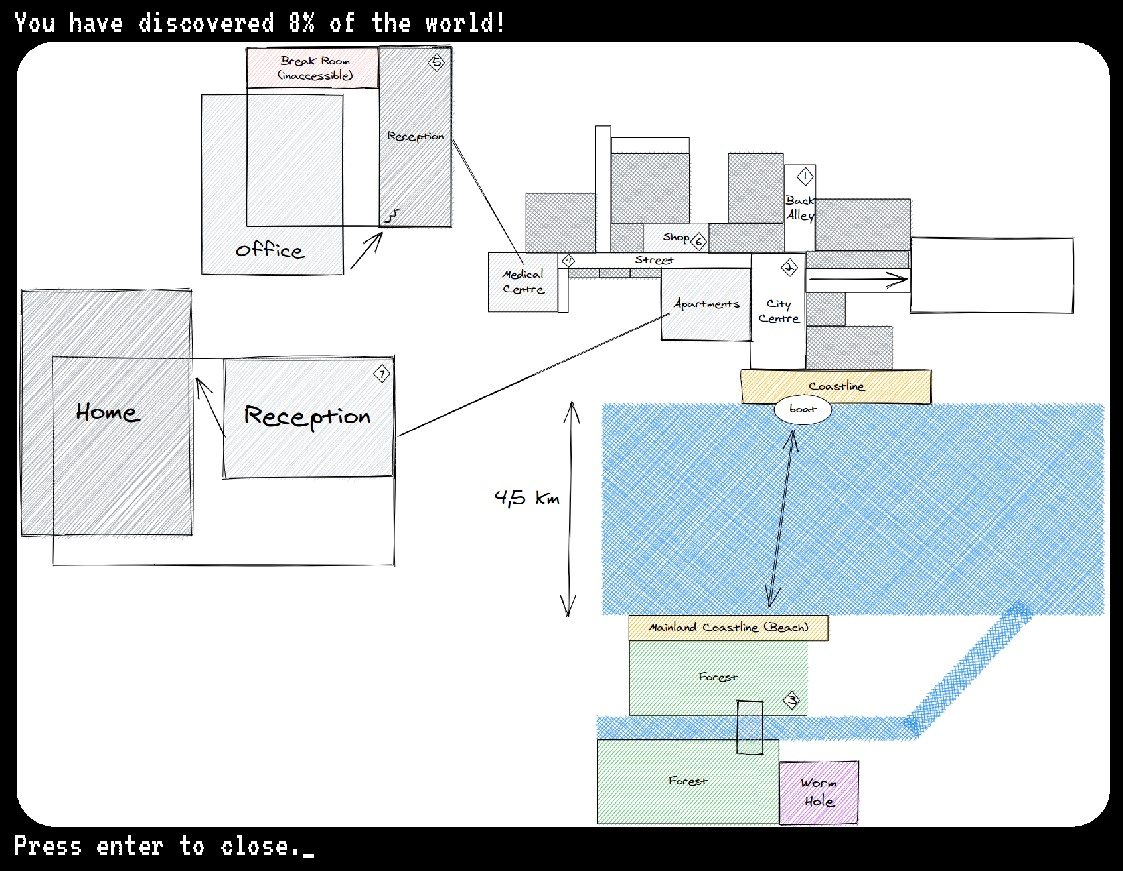
\includegraphics[width=\textwidth]{images/map-ingame.jpg}
        \caption{Output from the map command} \label{fig:map-ingame}
    \end{figure}
    \begin{figure}
        \lstinputlisting[language=Java]
        {../src/main/java/uk/insrt/coursework/zuul/events/Event.java}
        \caption{Event.java (uk.insrt.coursework.zuul.events.Event)} \label{fig:event}
    \end{figure}
    \begin{figure}
        \lstinputlisting[language=Java]
        {../src/main/java/uk/insrt/coursework/zuul/io/IOSystem.java}
        \caption{IOSystem.java (uk.insrt.coursework.zuul.io.IOSystem)} \label{fig:io-system}
    \end{figure}
    \begin{figure}
        \lstinputlisting[language=Java]
        {../src/main/java/uk/insrt/coursework/zuul/io/StandardIO.java}
        \caption{StandardIO.java (uk.insrt.coursework.zuul.io.StandardIO)} \label{fig:standard-io}
    \end{figure}
    \begin{figure}
        \lstinputlisting[language=Java]
        {../src/main/java/uk/insrt/coursework/zuul/io/LocalisedIO.java}
        \caption{LocalisedIO.java (uk.insrt.coursework.zuul.io.LocalisedIO)} \label{fig:localised-io}
    \end{figure}
    \begin{figure}
        \lstinputlisting[language=Java]
        {../src/main/java/uk/insrt/coursework/zuul/events/EventSystem.java}
        \caption{EventSystem.java (uk.insrt.coursework.zuul.events.EventSystem)} \label{fig:event-system}
    \end{figure}
    \begin{figure}
        \lstinputlisting[language=Java]
        {../src/main/java/uk/insrt/coursework/zuul/dialogue/DialogueOption.java}
        \caption{DialogueOption.java (uk.insrt.coursework.zuul.dialogue.DialogueOption)} \label{fig:dialogue}
    \end{figure}
    \begin{figure}
        \lstinputlisting[language=Java]
        {../src/main/java/uk/insrt/coursework/zuul/ui/EventDraw.java}
        \caption{EventDraw.java (uk.insrt.coursework.zuul.ui.EventDraw)} \label{fig:event-draw}
    \end{figure}
    \begin{figure}
        \begin{lstlisting}[language=Java]
public<E extends Event> void addListener(Class<E> event,
    IEventListener<E> listener) {
    this.getList(event).add(listener);
}\end{lstlisting}
        \caption{Excerpt from EventSystem.java (uk.insrt.coursework.zuul.events.EventSystem)} \label{fig:generic-method}
    \end{figure}
    \begin{figure}
        \begin{lstlisting}[language=Java]
/**
 * Get the current weight of this inventory.
 * @return Weight (in kg)
 */
public double getWeight() {
    return this
        .items
        .stream()
        .mapToDouble(Entity::getWeight)
        .sum();
}

/**
 * Check if the inventory is full.
 * @return True if the weight is greater than the max weight
 */
public boolean isFull() {
    return this.getWeight() >= this.getMaxWeight();
}

/**
 * Add an entity to this inventory.
 * 
 * There must be sufficient space for the entity.
 * @param entity Target Entity
 * @return Whether we successfully added the new entity.
 */
public boolean add(Entity entity) {
    if (this.getWeight() + entity.getWeight() > this.maxWeight) {
        return false;
    }

    this.items.add(entity);
    return true;
}\end{lstlisting}
        \caption{Excerpt from Inventory.java (uk.insrt.coursework.zuul.entities.Inventory)} \label{fig:inventory}
    \end{figure}
    \begin{figure}
        \begin{lstlisting}[language=Java]
/**
 * Write a string value to the text buffer.
 * @param value String value to write
 */
public void write(String value) {
    // Write each character sequentially.
    for (int i=0;i<value.length();i++) {
        char c = value.charAt(i);

        // If we encounter an Ansi escape character, then take the
        // substring from this point on and determine if it is a valid
        // escape code. If it is, apply any changes before continuing.
        if (c == '\u001B') {
            Matcher matcher = Ansi.AnsiPattern.matcher(value.substring(i));
            if (matcher.find()) {
                int v = Integer.parseInt(matcher.group(1));
                i += 3 + (v > 9 ? 1 : 0);

                if (v == 0) {
                    this.bg = Color.BLACK;
                    this.fg = Color.WHITE;
                } else if (v >= 30 && v < 38) {
                    this.fg = Ansi.fromEscapeCode(v);
                } else if (v >= 40 && v < 48) {
                    this.bg = Ansi.fromEscapeCode(v);
                }

                continue;
            }
        }

        this.write(c);
    }
}\end{lstlisting}
        \caption{Excerpt from TextBuffer.java (uk.insrt.coursework.zuul.ui.TextBuffer)} \label{fig:ansi-match}
    \end{figure}
\end{document}
